\documentclass[12pt]{article}

% Put your name/s and ID number/s here
\newcommand{\myname}{Waleed Lugod}
\newcommand{\myidnumber}{223798}
\newcommand{\mysection}{K}
 
% Put the problem set number here
\newcommand{\psetnumber}{4}

\usepackage{probset}
\usepackage{enumitem}

\setenumerate[0]{label=(\alph*)}
\usetikzlibrary{graphs}

\begin{document}
\problem{1}
\begin{enumerate}
	\item \hfill \\
		\begin{minipage}{0.45\textwidth}
			\centering
			\textbf{G1}\par\medskip
			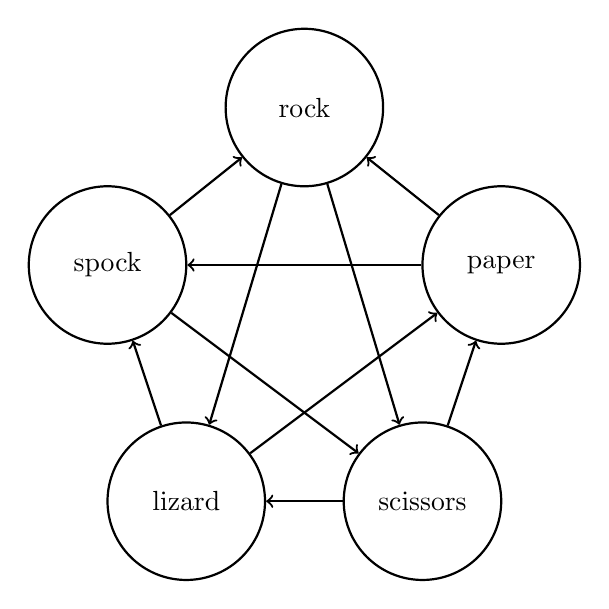
\begin{tikzpicture}
				[main/.style = {draw, circle,
				minimum size=20mm}, node distance={40mm},
				thick]
				\node[main] (rock) at (0, 2) {rock};
				\node[main] (paper) at (2.5, 0) {paper};
				\node[main] (scissors) at (1.5, -3) {scissors};
				\node[main] (lizard) at (-1.5, -3) {lizard};
				\node[main] (spock) at (-2.5, 0) {spock};
				\draw[->] (rock) -- (scissors);
				\draw[->] (rock) -- (lizard);
				\draw[->] (paper) -- (rock);
				\draw[->] (paper) -- (spock);
				\draw[->] (scissors) -- (paper);
				\draw[->] (scissors) -- (lizard);
				\draw[->] (lizard) -- (paper);
				\draw[->] (lizard) -- (spock);
				\draw[->] (spock) -- (rock);
				\draw[->] (spock) -- (scissors);
			\end{tikzpicture}
		\end{minipage}
		\begin{minipage}{0.5\textwidth}
			\centering
			\textbf{G2}\par\medskip
			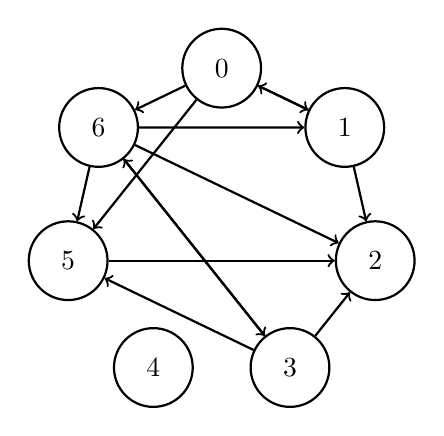
\begin{tikzpicture}
				[main/.style = {draw, circle,
				minimum size=10mm}, thick]
				\pgfmathsetmacro\n{7}
				\foreach \i in {0, 1, 2, 3, 4, 5, 6} {
					\pgfmathsetmacro\r{\i*(360/-\n)+90}
					\node[main] (\i) at (\r:2) {\i};
				}
				\draw[->] (0) -- (1);
				\draw[->] (0) -- (5);
				\draw[->] (0) -- (6);
				\draw[->] (1) -- (0);
				\draw[->] (1) -- (2);
				\draw[->] (3) -- (6);
				\draw[->] (3) -- (2);
				\draw[->] (3) -- (5);
				\draw[->] (5) -- (2);
				\draw[->] (6) -- (1);
				\draw[->] (6) -- (2);
				\draw[->] (6) -- (3);
				\draw[->] (6) -- (5);
			\end{tikzpicture}
		\end{minipage}
	\item \hfill \\
		\begin{tikzpicture}
		\end{tikzpicture}
\end{enumerate}
\end{document}
